\documentclass{article}

\usepackage[T1]{fontenc}
\usepackage[paperwidth=19.4cm,paperheight=15.7cm,margin=0.35cm]{geometry}
\usepackage[scaled=0.95]{helvet}
\renewcommand{\familydefault}{\sfdefault}
\usepackage{amsmath}
\usepackage{graphicx}
\usepackage{tikz}
\usetikzlibrary{arrows.meta,calc,positioning}

\definecolor{navy}{RGB}{31,42,68}
\definecolor{slate}{RGB}{103,112,133}
\definecolor{panelstroke}{RGB}{216,221,230}
\definecolor{boxfill}{RGB}{249,250,252}

\newcommand{\figtitle}[1]{%
  {\color{navy}\fontsize{13.4}{15.8}\selectfont\bfseries #1}%
}
\newcommand{\panellabel}[1]{%
  {\color{navy}\fontsize{11.6}{13.4}\selectfont\bfseries #1}%
}
\newcommand{\paneltitle}[1]{%
  {\color{navy}\fontsize{10.9}{12.8}\selectfont\bfseries #1}%
}
\newcommand{\panelsubtitle}[1]{%
  {\color{slate}\fontsize{8.4}{10.2}\selectfont #1}%
}
\newcommand{\boxtitle}[1]{%
  {\color{navy}\fontsize{9.6}{11.5}\selectfont\bfseries #1}%
}
\newcommand{\boxsubtitle}[1]{%
  {\color{navy}\fontsize{8.2}{9.9}\selectfont #1}%
}
\newcommand{\boxeqn}[1]{%
  {\color{slate}\fontsize{9.3}{11.0}\selectfont #1}%
}
\newcommand{\vignettelabel}[1]{%
  {\color{slate}\fontsize{7.1}{8.4}\selectfont\bfseries #1}%
}

% External asset hooks.
% Prefer vector PDFs where available; only these filenames need to change.
\newcommand{\qfile}{schematic_q.png}
\newcommand{\pfile}{schematic_p.png}
\newcommand{\tfpfile}{schematic_tfp.pdf}
\newcommand{\panelBfile}{g_ribbon_intervals_KLEMS.jpeg}
\newcommand{\panelCfile}{g_error_hulten_quantiles.jpeg}

\newcommand{\panelimageplaceholder}[2]{%
  \begin{tikzpicture}[x=1cm,y=1cm]
    \draw[panelstroke, rounded corners=2.4pt, line width=0.45pt, fill=boxfill] (0,0) rectangle (#1,#2);
    \draw[panelstroke, line width=0.38pt] (0.34,0.34) -- (#1-0.34,#2-0.34);
    \draw[panelstroke, line width=0.38pt] (0.34,#2-0.34) -- (#1-0.34,0.34);
    \node[text=slate, align=center, font=\fontsize{8.2}{9.8}\selectfont] at (#1/2,#2/2)
      {Insert external plot};
  \end{tikzpicture}%
}

\newcommand{\panelgraphictrimmed}[4]{%
  \IfFileExists{#1}{%
    \includegraphics[width=#2,height=#3,keepaspectratio,clip,trim=#4]{#1}%
  }{%
    \panelimageplaceholder{#2}{#3}%
  }%
}

\newcommand{\vignetteplaceholder}[3]{%
  \begin{tikzpicture}[x=1cm,y=1cm]
    \draw[panelstroke, rounded corners=2.4pt, line width=0.40pt, fill=white] (0,0) rectangle (#1,#2);
    \node[text=slate, align=center, font=\fontsize{7.0}{8.4}\selectfont] at (#1/2,#2/2) {#3};
  \end{tikzpicture}%
}

\newcommand{\vignettegraphic}[4]{%
  \IfFileExists{#1}{%
    \includegraphics[width=#2,height=#3,keepaspectratio]{#1}%
  }{%
    \vignetteplaceholder{#2}{#3}{#4}%
  }%
}

\begin{document}
\thispagestyle{empty}
\pagestyle{empty}
\noindent
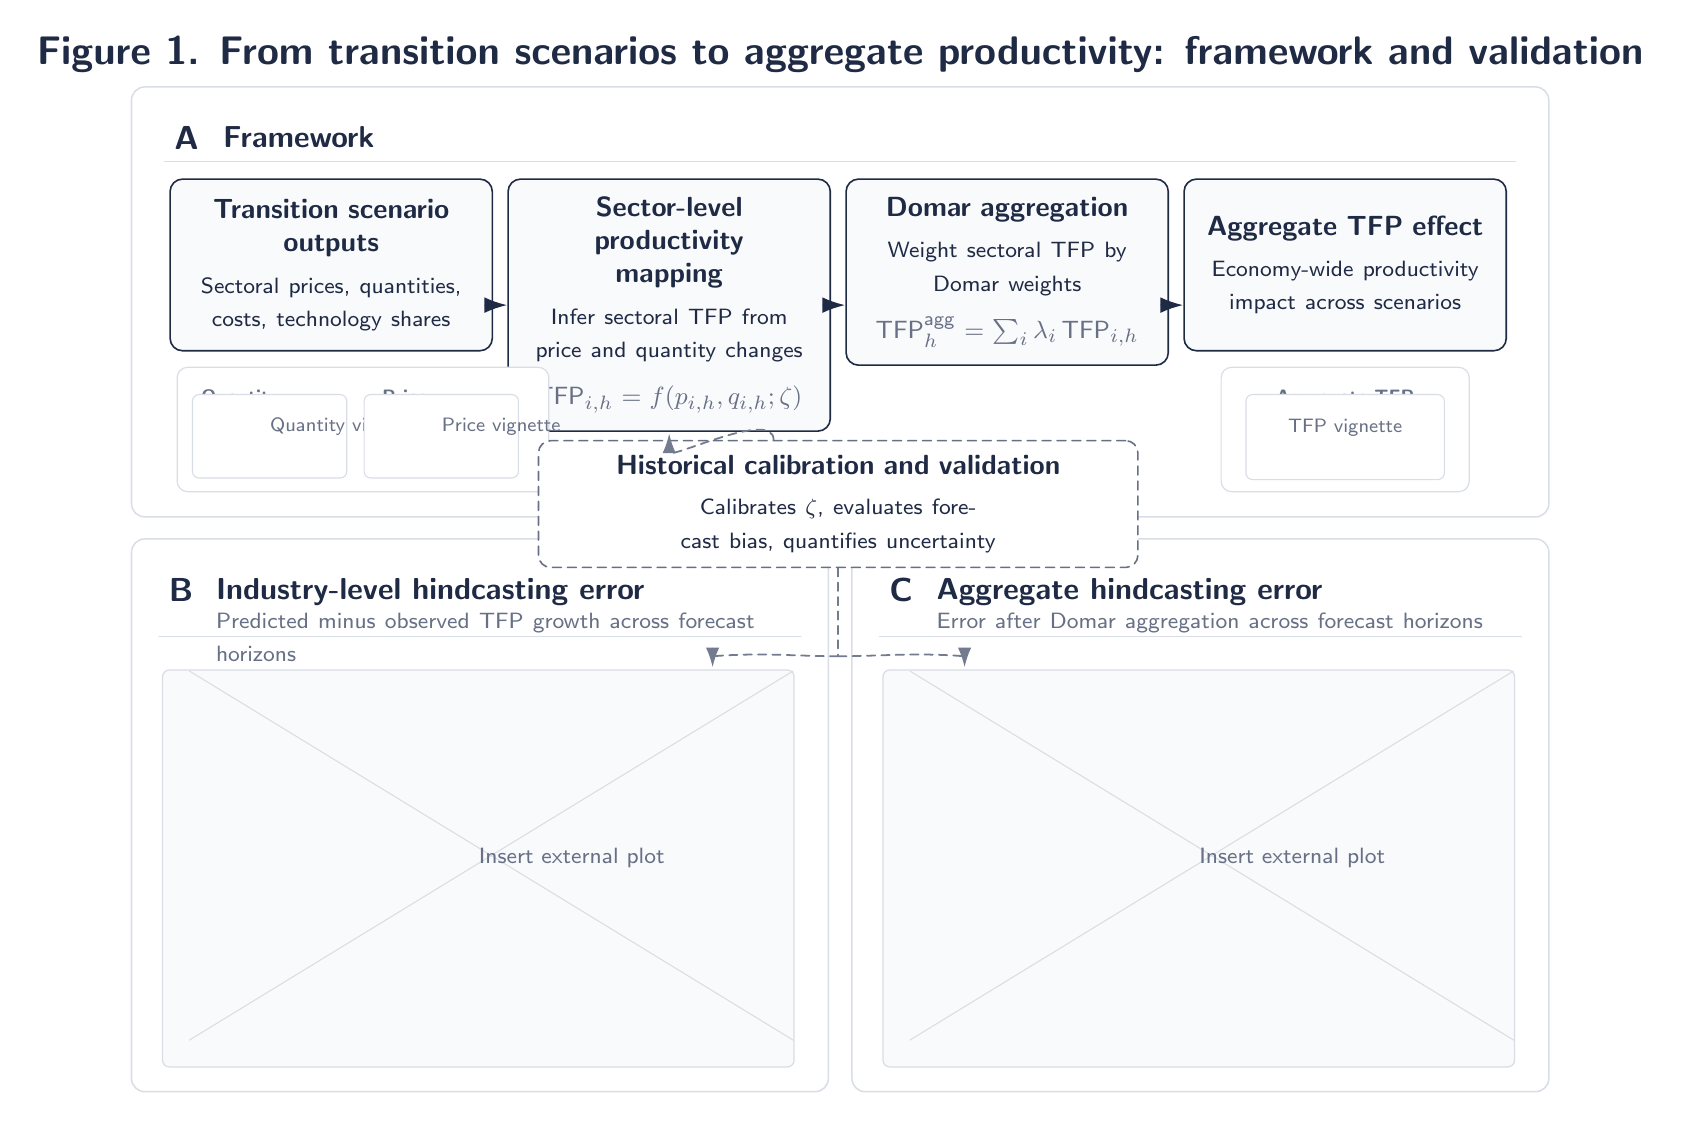
\begin{tikzpicture}[x=1cm,y=1cm,>=Latex,line cap=round,line join=round]

\tikzset{
  panel/.style={
    draw=panelstroke,
    rounded corners=4.8pt,
    line width=0.55pt,
    fill=white,
    inner sep=0pt,
    outer sep=0pt
  },
  workflowbox/.style={
    draw=navy,
    rounded corners=4.5pt,
    line width=0.58pt,
    fill=boxfill,
    align=center,
    text width=3.60cm,
    minimum height=2.18cm,
    inner xsep=7pt,
    inner ysep=6.5pt
  },
  vignettegroup/.style={
    draw=panelstroke,
    rounded corners=3.8pt,
    line width=0.42pt,
    fill=white,
    inner sep=0pt,
    outer sep=0pt
  },
  bridgebox/.style={
    draw=slate,
    rounded corners=4.4pt,
    dash pattern=on 3.2pt off 2.2pt,
    line width=0.58pt,
    fill=white,
    align=center,
    text width=7.05cm,
    minimum height=0.96cm,
    inner xsep=8pt,
    inner ysep=5.4pt
  },
  mainflow/.style={
    -{Latex[length=2.9mm,width=2.0mm]},
    draw=navy,
    line width=0.82pt
  },
  bridgepath/.style={
    draw=slate!92,
    dash pattern=on 3.0pt off 2.2pt,
    line width=0.64pt
  },
  bridgearrow/.style={
    -{Latex[length=2.5mm,width=1.7mm]},
    draw=slate!92,
    dash pattern=on 3.0pt off 2.2pt,
    line width=0.64pt
  }
}

% Figure title
\node[anchor=north] at (9,-0.12)
  {\figtitle{Figure 1. From transition scenarios to aggregate productivity: framework and validation}};

% Overall panel frames
\node[panel, minimum width=18.00cm, minimum height=5.46cm, anchor=north west] (panelA) at (0,-0.88) {};
\node[panel, minimum width=8.85cm, minimum height=7.02cm, anchor=north west]  (panelB) at (0,-6.62) {};
\node[panel, minimum width=8.85cm, minimum height=7.02cm, anchor=north west]  (panelC) at (9.15,-6.62) {};

% Panel headers
\node[anchor=north west] at ($(panelA.north west)+(0.42,-0.38)$) {\panellabel{A}};
\node[anchor=north west] at ($(panelA.north west)+(1.04,-0.38)$) {\paneltitle{Framework}};
\draw[panelstroke, line width=0.45pt]
  ($(panelA.north west)+(0.42,-0.95)$) -- ($(panelA.north east)+(-0.42,-0.95)$);

\node[anchor=north west] at ($(panelB.north west)+(0.35,-0.38)$) {\panellabel{B}};
\node[anchor=north west] at ($(panelB.north west)+(0.95,-0.38)$) {\paneltitle{Industry-level hindcasting error}};
\node[anchor=north west, align=left, text width=7.28cm]
  at ($(panelB.north west)+(0.95,-0.82)$)
  {\panelsubtitle{Predicted minus observed TFP growth across forecast horizons}};
\draw[panelstroke, line width=0.45pt]
  ($(panelB.north west)+(0.35,-1.24)$) -- ($(panelB.north east)+(-0.35,-1.24)$);

\node[anchor=north west] at ($(panelC.north west)+(0.35,-0.38)$) {\panellabel{C}};
\node[anchor=north west] at ($(panelC.north west)+(0.95,-0.38)$) {\paneltitle{Aggregate hindcasting error}};
\node[anchor=north west, align=left, text width=7.28cm]
  at ($(panelC.north west)+(0.95,-0.82)$)
  {\panelsubtitle{Error after Domar aggregation across forecast horizons}};
\draw[panelstroke, line width=0.45pt]
  ($(panelC.north west)+(0.35,-1.24)$) -- ($(panelC.north east)+(-0.35,-1.24)$);

% Panel A: workflow row
\coordinate (workflowNW) at ($(panelA.north west)+(0.48,-1.16)$);

\node[workflowbox, anchor=north west] (b1) at (workflowNW) {%
  \boxtitle{Transition scenario}\\
  \boxtitle{outputs}\\[3pt]
  \boxsubtitle{Sectoral prices, quantities,}\\
  \boxsubtitle{costs, technology shares}
};

\node[workflowbox, anchor=north west] (b2) at ($(b1.north east)+(0.18,0)$) {%
  \boxtitle{Sector-level productivity}\\
  \boxtitle{mapping}\\[3pt]
  \boxsubtitle{Infer sectoral TFP from}\\
  \boxsubtitle{price and quantity changes}\\[5pt]
  \boxeqn{$\mathsf{TFP}_{i,h}=f(p_{i,h},q_{i,h};\zeta)$}
};

\node[workflowbox, anchor=north west] (b3) at ($(b2.north east)+(0.18,0)$) {%
  \boxtitle{Domar aggregation}\\[3pt]
  \boxsubtitle{Weight sectoral TFP by}\\
  \boxsubtitle{Domar weights}\\[5pt]
  \boxeqn{$\mathsf{TFP}^{\text{agg}}_h=\sum_i \lambda_i\,\mathsf{TFP}_{i,h}$}
};

\node[workflowbox, anchor=north west] (b4) at ($(b3.north east)+(0.18,0)$) {%
  \boxtitle{Aggregate TFP effect}\\[3pt]
  \boxsubtitle{Economy-wide productivity}\\
  \boxsubtitle{impact across scenarios}
};

\coordinate (flowaxis) at (b2.center);
\draw[mainflow] ($(b1.east |- flowaxis)$) -- ($(b2.west |- flowaxis)$);
\draw[mainflow] ($(b2.east |- flowaxis)$) -- ($(b3.west |- flowaxis)$);
\draw[mainflow] ($(b3.east |- flowaxis)$) -- ($(b4.west |- flowaxis)$);

% Panel A: deliberate vignette row
\node[vignettegroup, minimum width=4.72cm, minimum height=1.58cm, anchor=north west] (vleft)
  at ($(b1.south west)+(0.10,-0.20)$) {};
\node[anchor=north west] at ($(vleft.north west)+(0.18,-0.16)$) {\vignettelabel{Quantity}};
\node[anchor=north west] at ($(vleft.north west)+(2.48,-0.16)$) {\vignettelabel{Price}};
\node[anchor=south west, inner sep=0pt] at ($(vleft.south west)+(0.18,0.16)$)
  {\vignettegraphic{\qfile}{1.96cm}{1.06cm}{Quantity vignette}};
\node[anchor=south west, inner sep=0pt] at ($(vleft.south west)+(2.36,0.16)$)
  {\vignettegraphic{\pfile}{1.96cm}{1.06cm}{Price vignette}};

\node[vignettegroup, minimum width=3.15cm, minimum height=1.58cm, anchor=north] (vright)
  at ($(b4.south)+(0,-0.20)$) {};
\node[anchor=north] at ($(vright.north)+(0,-0.16)$) {\vignettelabel{Aggregate TFP}};
\node[anchor=south, inner sep=0pt] at ($(vright.south)+(0,0.14)$)
  {\vignettegraphic{\tfpfile}{2.52cm}{1.08cm}{TFP vignette}};

% Panel A: central validation bridge
\node[bridgebox, anchor=north] (backtest)
  at ($(b2.south)!0.5!(b3.south)+(0,-0.52)$) {%
    \boxtitle{Historical calibration and validation}\\[2.5pt]
    \boxsubtitle{Calibrates $\zeta$, evaluates forecast bias, quantifies uncertainty}
  };

\draw[bridgearrow]
  ($(backtest.north)+(-0.82,0)$)
  .. controls +(0,0.40) and +(0,-0.34) ..
  ($(b2.south)+(0,-0.02)$);

% Imported empirical plots. Swap the file hooks above to PDF assets when available.
\node[anchor=south west, inner sep=0pt] (plotB)
  at ($(panelB.south west)+(0.38,0.30)$)
  {\panelgraphictrimmed{\panelBfile}{8.02cm}{5.04cm}{18pt 38pt 14pt 158pt}};

\node[anchor=south west, inner sep=0pt] (plotC)
  at ($(panelC.south west)+(0.38,0.30)$)
  {\panelgraphictrimmed{\panelCfile}{8.02cm}{5.04cm}{18pt 34pt 14pt 158pt}};

% Downstream dashed links to the validation evidence panels
\coordinate (validationFork) at ($(backtest.south)+(0,-0.28)$);
\coordinate (plotBridgeLevel) at ($(plotB.north)+(0,0.16)$);
\coordinate (bridgeLevel) at (validationFork |- plotBridgeLevel);
\coordinate (bridgeB) at ($(plotB.north east)+(-1.05,0.16)$);
\coordinate (bridgeC) at ($(plotC.north west)+(1.05,0.16)$);

\draw[bridgepath] (backtest.south) -- (validationFork) -- (bridgeLevel);
\draw[bridgepath]
  (bridgeLevel) .. controls +(-0.52,0) and +(0.62,0.05) .. (bridgeB);
\draw[bridgepath]
  (bridgeLevel) .. controls +(0.52,0) and +(-0.62,0.05) .. (bridgeC);
\draw[bridgearrow] (bridgeB) -- ($(plotB.north east)+(-1.05,0.02)$);
\draw[bridgearrow] (bridgeC) -- ($(plotC.north west)+(1.05,0.02)$);

\end{tikzpicture}
\end{document}
